\documentclass{article}
\usepackage[utf8]{inputenc}          % Italian accents
\usepackage[english]{babel}
\usepackage{graphicx}    
\usepackage{amsmath}                 
\usepackage{amsfonts}                
\usepackage{amssymb}    
% extra math symbols             
\usepackage{mathrsfs}                 
\usepackage{bm}
\usepackage{color}
\definecolor{mygreen}{rgb}{0,0.6,0}
\definecolor{mygray}{rgb}{0.5,0.5,0.5}
\definecolor{mymauve}{rgb}{0.58,0,0.82}
% for including source code snippet
\usepackage{listings}
\usepackage[font=small,it]{caption} % differentiate captions from normal text
\usepackage{hyperref} %for using autoref

\lstset{ 
	backgroundcolor=\color{white},   % choose the background color; you must add \usepackage{color} or \usepackage{xcolor}; should come as last argument
	basicstyle=\scriptsize,          % the size of the fonts that are used for the code \scriptsize
	breakatwhitespace=false,         % sets if automatic breaks should only happen at whitespace
	breaklines=true,                 % sets automatic line breaking
	captionpos=b,                    % sets the caption-position to bottom
	commentstyle=\color{mygreen},    % comment style
	deletekeywords={...},            % if you want to delete keywords from the given language
	escapeinside={\%*}{*)},          % if you want to add LaTeX within your code
	extendedchars=true,              % lets you use non-ASCII characters; for 8-bits encodings only, does not work with UTF-8
	float=htpb,                        % floating behaviour  
	frame=single,                    % adds a frame around the code
	keepspaces=true,                 % keeps spaces in text, useful for keeping indentation of code (possibly needs columns=flexible)
	keywordstyle=\color{blue},       % keyword style
	language=C++,                % the language of the code
	morekeywords={*,...},            % if you want to add more keywords to the set
	numbers=left,                    % where to put the line-numbers; possible values are (none, left, right)
	numbersep=5pt,                   % how far the line-numbers are from the code
	numberstyle=\tiny\color{mygray}, % the style that is used for the line-numbers
	rulecolor=\color{black},         % if not set, the frame-color may be changed on line-breaks within not-black text (e.g. comments (green here))
	showspaces=false,                % show spaces everywhere adding particular underscores; it overrides 'showstringspaces'
	showstringspaces=false,          % underline spaces within strings only
	showtabs=false,                  % show tabs within strings adding particular underscores
	stepnumber=2,                    % the step between two line-numbers. If it's 1, each line will be numbered
	stringstyle=\color{mymauve},     % string literal style
	tabsize=2,                       % sets default tabsize to 2 spaces
	title=\lstname                   % show the filename of files included with \lstinputlisting; also try caption instead of title
}

\begin{document} 
	
	\author{Cesare Cozza \\ Prisco Lo Chiatto }
	\title{Numerical simulation of the longitudinal dispersion bands of phonons in a $(GaAs)_1/(AlAs)_1$ superlattice}
	
	\maketitle
    \newpage
    
    
\section{Abstract}




\section{Introduction}
\begin{figure}
	\centering
	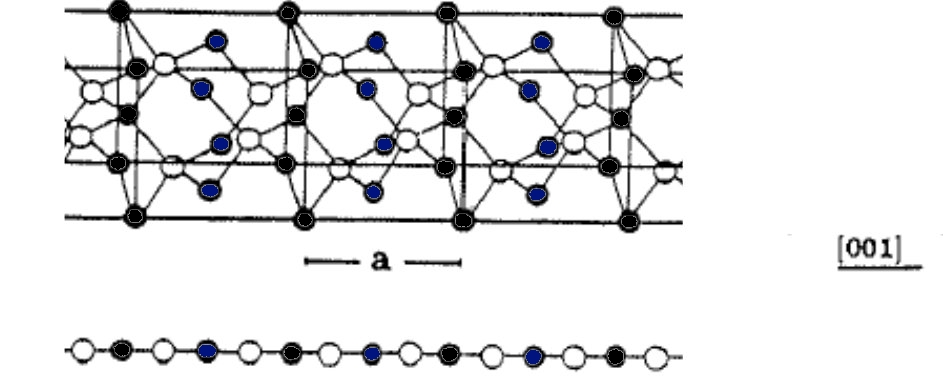
\includegraphics[scale=0.3]{reticolo.jpg}
	\caption{The superlattice used in this study and its projection on the [001] direction. Gallium atoms are painted black, Aluminium ones are blue and Arsenic is white. Note that, while projectin on the [001] direction, the motion of each one of the planes can be inferred from a single atom model.}
	\label{fig:reticolo}
\end{figure}
The scope of this work is to study the longitudinal vibrational properties of a $(GaAs)_1/(AlAs)_1$ superlattice trough a simple numerical simulation.\medskip

A superlattice is a kind of metamaterial made up from two (or more) materials, in a periodic structure. An ideal $(GaAs)_1/(AlAs)_1$ superlattice is made up from one layer of $GaAs$ followed by one of $AlAs$ in a periodic matter (see \autoref{fig:reticolo}.\smallskip

	In general, the vibrational properties of a crystalline solid can be studied trough lattice dynamics; thanks to the periodicity of the system the problem can be further reduced to the solution of the dynamics of the atoms in the unitary cell.\\
	Three more approximations will be employed:
	\begin{enumerate}
		\item \textbf{The harmonic approximation}, which consider the atomics cores as simple harmonic oscillator
		\item \textbf{The first neighbour approximation}, where for each atom the interaction between anything other than the closest atoms next to it are neglected.
		\item \textbf{The Born-Oppenheimer approximation} where ionic and electronic motions can be treated indipendently.
	\end{enumerate}
	Thanks to these approximation it is possible to treat in a simple manner the quanto-mechanical problem of vibration in a solid and find the dispersion bands (how the frequency depends on $\vec{q}$, the wavevector of the phonon).\\
Normal vibrational modes of a of quantized elastic system are called phonon. They are collective excitation - i.e. bosonic quasiparticles - and their dispersion relation are related to a number of properties of the system itself. \smallskip 

\begin{figure}
	\centering
	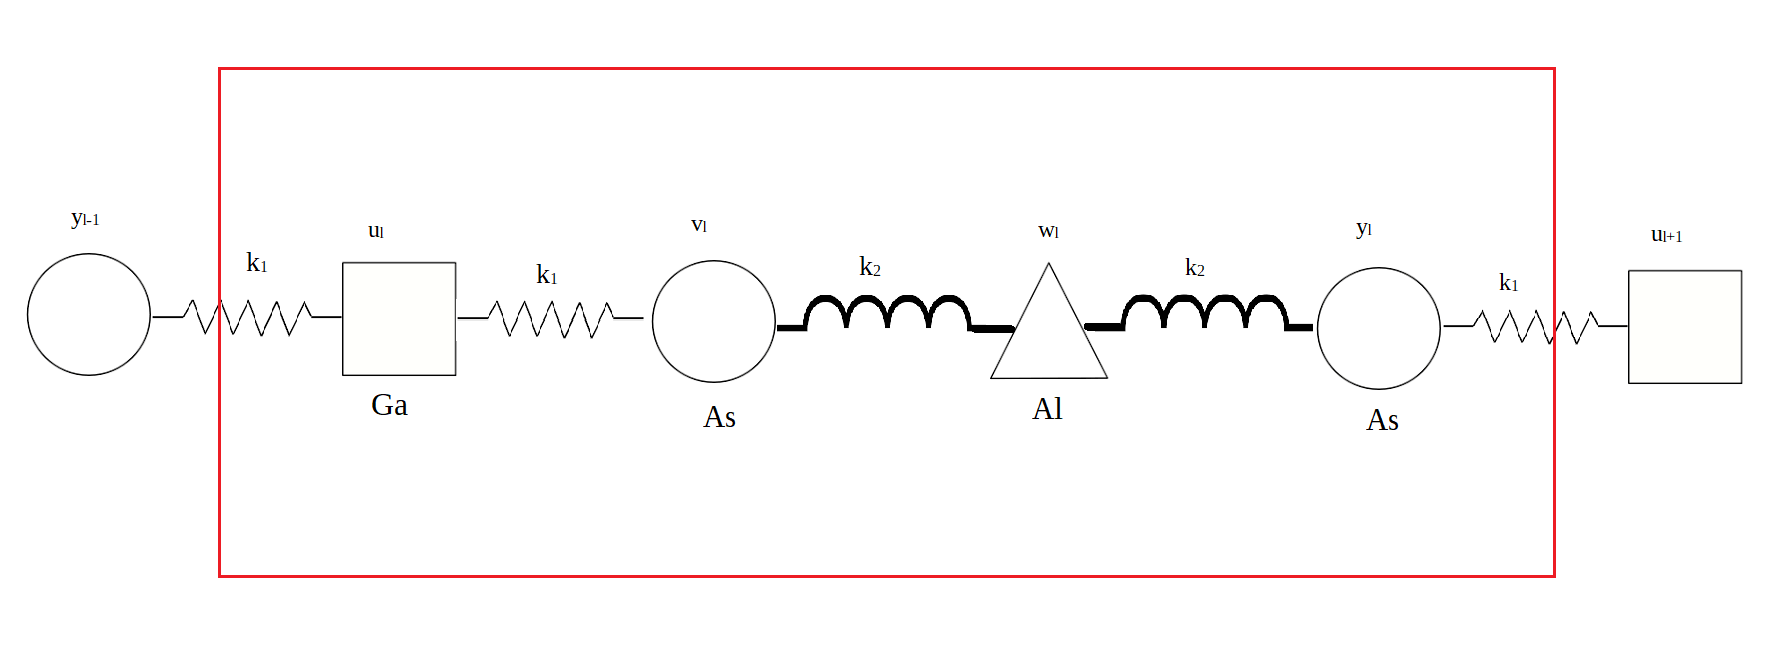
\includegraphics[width=0.7\linewidth]{cella.png}
	\caption{The 4-atom unitary cell analysed in this work.\\
	$k_1$ is the elastic constant between $Ga$ and $As$ and $k_2$ is the elastic constant between $Al$ and $As$. Considering an infinite linear chain $u_l$ represent the displacement of the l-th (arbitrary origin) atom of $Ga$, $v_l$ the displacement of the l-th atom of $As$ of the GaAs molecule, $w_l$ the displacement of the l-th atom of $Al$, $y_l$ the displacement of the l-th atom of $As$ of the $AlAs$ molecule.   }
	\label{fig:cella}
\end{figure}

The [0,0,1] direction has been considered, so that the materials' layers follow each other orthogonally with respect to this direction. Only longitudinal vibrations have been taken into account. \\
Thanks to the periodicity of the system and the approximations taken each layer will be considered as a single atom (see \autoref{fig:reticolo}). The physical model is then a linear chain of atoms in which the unit cell is made up by 4 atoms, $Ga$-$As$-$Al$-$As$ as in \autoref{fig:cella}, and only interaction with first neighbour has been taken into account. \\
Thanks to the harmonic approximation it is possible to solve the dynamic of the system using Hooke's Law and considering the displacement of each atom with respect to its equilibrium position.The following system results (see \autoref{fig:cella} for the meaning of each symbol):
\begin{equation}
	\begin{cases}
	M_{Ga}\ddot{u_l} = -k_1(u_l-v_l) - k_1(u_l-y_{l-1}) \\
	M_{As}\ddot{v_l} = -k_1(v_l-u_l) - k_2(v_l-w_l) \\
	M_{Al}\ddot{w_l} = -k_2(w_l-v_l) - k_2(w_l-y_l) \\
	M_{As}\ddot{y_l} = -k_2(y_l-w_l) - k_1(y_l-u_{l+1}) \\
	\end{cases}
	\label{eq:sistema}	
\end{equation}
To solve this system we impose that every displacement has the form of a plane wave:
\begin{equation}
	\begin{cases}
	u_l = Ue^{i(qla-\omega t)} \\
	v_l = Ve^{i(qla-\omega t)} \\
	w_l = We^{i(qla-\omega t)} \\
	y_l = Ye^{i(qla-\omega t)} \\
	\end{cases}
	\label{eq:onde piane}
\end{equation}
where $a$ is the lattice parameter of the superlattice (sum of the lengths of the respective unit cells).
Solving the system for $\omega$ and then varying $\vec{q}$ will lead to the dispersion bands; because the unit cell has 4 atoms the system to solve is 4-dimensional and so 4 dispersion bands are expected.  




\section{Numerical solution}
The problem of the dispersion bads of GaAs/AlAs reduces to the solution of the system showed in \autoref{eq:sistema}. \\
Substituting in the system the solution for the plain wave in \autoref{eq:onde piane}, after some algebra one gets:
\begin{equation}
	\begin{cases}
	(-\omega^2M_1 + 2k_1)U - k_1V - (k_1e^{-iqa})Y = 0 \\
    (-\omega^2M_3 + 2K2)W -k_2V - k_2Y = 0 \\
	-k_1U -k_2W + (-\omega^2M_2 + k_1 + k_2)V = 0 \\
	-(k_1e^{iqa})U - k_2W + (-\omega^2M_2 + k_1 + k_2)Y = 0	
	\end{cases}
	\label{sist.final}
\end{equation}
This is convenient as the system's associated matrix is already written in the form $[-\omega^2I + A]$, where


\begin{equation} 
A = \begin{pmatrix}
   \frac{2k_1}{M_{Ga}}	& 0  & -\frac{k_1}{M_{Ga}}  & -\frac{k_1}{M_{Ga}}e^{-iqa}  \\ 
   0	& \frac{2k_2}{M_{Al}}  & -\frac{k_2}{M_{Al}}  & -\frac{k_2}{M_{Al}}  \\ 
   -\frac{k_1}{M_{As}} 	& -\frac{k_2}{M_{As}}   & \frac{k_1}{M_{As}}+\frac{k_2}{M_{As}}   & 0  \\ 
   -\frac{k_1}{M_{As}}e^{iqa} 	& -\frac{k_2}{M_{As}}  & 0  & \frac{k_1}{M_{As}}+\frac{k_2}{M_{As}}   
\end{pmatrix} 
\label{eq:matrice}
\end{equation}

so it is possible to solve the secular equation and find $\omega^2$. Varying $q$ inside the first Brillouin Zone one arrives at the dispersion relation. The eigenvectors of A are instead the displacement of the single atoms in the chain.\par
\medskip

To obtain the solution of the problem a numerical approach was undertaken: a program in C++ has been written which, after discretising the Brillouin Zone in a selected number of points, calculate appropriate wavevector $q$ for each points, and then fills the matrix in \autoref{eq:matrice} with the appropriate values. Finally, using a subroutine of the $Eigen$ linear algebra package, it finds eigenvectors and eigenvalues for each matrix.\\
The result is a discretized version of the dispersion relation, which is then plotted with GNUPLOT.

\begin{lstlisting}[language=C++, caption={Subroutine norma \\ \emph{maodulo.f90}}]

CODICE

\end{lstlisting} 


	

\end{document}
